\chapter{Testentwurf}

Der allgemeine Testentwurf besteht aus zwei einzelnen Phasen.
In der ersten Phase wird das GraphQL Schema analysiert und die Prime-Paths generiert.
So haben wir grundlegendes Wissen darüber, welche Querys ausgeführt werden müssen damit jeder Bereich
der API abgedeckt ist.
In der zweiten Phase \ldots

\section{erste Phase / GraphQL Analyse}

Grundlage der Analyse einer GraphQL-API ist ihr Schema.
Die gesamte erste Phase bezieht sich nur auf das Schema denn aus diesem können wir alle grundlegenden
Test-Cases ermitteln die nötig sind um eine Überdeckung der Anfragen zu ermitteln.
Es sei hier gesagt, dass nur die Überdeckung der Anfragen nicht bedeutet, dass die API hiermit vollständig getestet wird,
hierdurch werden nur alle Anfragen erstellt, sodass jeder Knoten und jede Kante im definierten Schema mindestens
einmal Betrachtung findet in einem Test.
Die dahinterliegenden Resolver benötigen weitere Abdeckung hierzu jedoch mehr in Phase 2.

\subsection{GraphQL in Graph übersetzen}

Um ein GraphQL Schema in einen Graphen zu übersetzen, bedarf es mehrerer Schritte.
Im GraphQL Standard implementiert jeder GraphQL-Client eine {\tt parse()} Funktion.
Diese werden wir auch nutzen, da wir hierdurch einen Graphen erhalten der für unsere Berechnungen auf dem
Graphen passend ist.
Die {\tt parse()} Funktion führt im wesentlichen zwei Schritte aus:

\begin{description}
    \item[Lexikalische Analyse] Schema in Token zerlegen
    \item[Syntaktische Analyse] Token in passende Graph-Repräsentation übersetzen
\end{description} (Quelle X.Y.Z)

Endergebnis ist ein Abstract Syntax Tree (AST) (Quelle einfügen).
Ein AST sieht je nach GraphQL-Client Plattform unterschiedlich, jedoch sehr ähnlich aus.
Folgendes, sehr simples Schema:

\begin{verbatim}
    type Query {
      user(id: Int): User
    }

    type User {
      id: Int
      name: String
    }
\end{verbatim}

wird in folgenden AST übersetzt (in Java-/Type-script ist der AST in json Format):

\begin{lstlisting}[language=json,firstnumber=1]
{
  "kind": "Document",
  "definitions": [
    {
      "kind": "ObjectTypeDefinition",
      "name": {
        "kind": "Name",
        "value": "Book"
      },
      "fields": [
        {
          "kind": "FieldDefinition",
          "name": {
            "kind": "Name",
            "value": "id"
          },
          "type": {
            "kind": "NamedType",
            "name": {
              "kind": "Name",
              "value": "Int"
            }
          }
        },
        {
          "kind": "FieldDefinition",
          "name": {
            "kind": "Name",
            "value": "title"
          },
          "type": {
            "kind": "NamedType",
            "name": {
              "kind": "Name",
              "value": "String"
            }
          }
        },
        {
          "kind": "FieldDefinition",
          "name": {
            "kind": "Name",
            "value": "author"
          },
          "type": {
            "kind": "NamedType",
            "name": {
              "kind": "Name",
              "value": "Author"
            }
          }
        }
      ]
    },
    {
      "kind": "ObjectTypeDefinition",
      "name": {
        "kind": "Name",
        "value": "Author"
      },
      "fields": [
        {
          "kind": "FieldDefinition",
          "name": {
            "kind": "Name",
            "value": "id"
          },
          "type": {
            "kind": "NamedType",
            "name": {
              "kind": "Name",
              "value": "Int"
            }
          }
        },
        {
          "kind": "FieldDefinition",
          "name": {
            "kind": "Name",
            "value": "name"
          },
          "type": {
            "kind": "NamedType",
            "name": {
              "kind": "Name",
              "value": "String"
            }
          }
        },
        {
          "kind": "FieldDefinition",
          "name": {
            "kind": "Name",
            "value": "written"
          },
          "type": {
            "kind": "ListType",
            "type": {
              "kind": "NonNullType",
              "type": {
                "kind": "NamedType",
                "name": {
                  "kind": "Name",
                  "value": "Books"
                }
              }
            }
          }
        }
      ]
    }
  ]
}

\end{lstlisting}

Die Ausgabe in diesem AST verrät uns für jede "ObjectTypeDefinition" das wir hier einen Knoten des Graphens haben
und in dem "Fields" eintrag kann man alle möglichen Verbindungen des Knotens finden.

\subsection{Pfadgenerierung}

Da wir im vorherigen Schritt eine geeignete Darstellung gefunden haben, um unseren Graphen zu repräsentieren können wir
nun im ersten Schritt alle Pfade ausgehend vom Querytype innerhalb dieses Graphens finden.
Um die Pfade zu ermitteln müssen wir lediglich wissen, welche Typen ein einzelner Knoten haben kann.
In Kapitel (GraphQL Kapitel verlinken) wurde bereits auf alle möglichen Typen eingegangen.
Hierbei sind für die Pfadgenerierung nur diese wichtig:
\begin{center}
  \begin{description}
    \item[FieldDefiniton]
    \item[NonNullType]
    \item[ListType]
    \item[ObjectTypeDefinition]
  \end{description} (Quelle X.Y.Z)
\end{center}

Aus unserem schon bekannten Schema:

\begin{verbatim}
type Book {
    id: Int
    title: String
    author: Author
}
type Author {
    id: Int
    name: String
    books: [Book]
}
type Query {
    # test query
    hello: String
    # all books
    books: [Book]
    # all authors
    authors: [Author]
    # a single book from a author name
    bookWrittenBy(name: String!): Book
    # all books from a author
    booksWrittenBy(name: String!): [Book]
    # a author for a book title
    writtenBy(title: String!): Author
}
\end{verbatim}

können wir nun beginnen die Pfade zu generieren. Hierbei müssen wir nur Pfade generieren, die ihren
Ursprung im Query Type haben denn andere Typen sind nicht initial abfragbar sondern nur durch Verkettung mit einer
Operation vom Query Type. Jedes Feld vom Query Type ist ein Einstiegspunkt für einen Pfad.
Ein Pfad führt weiter, wenn das Ergebnis eines Pfades eine ObjectTypeDefinition enthält. Also hier dementsprechend
"Author" oder "Book"

Besagtes Schema führt dann zu folgendem Graphen:

\begin{center}
  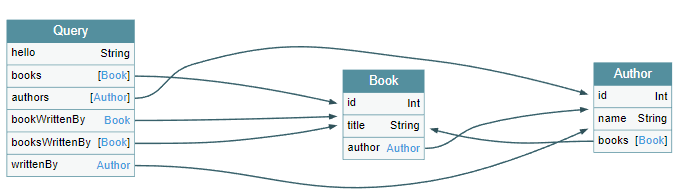
\includegraphics[width=\textwidth,height=\textheight,keepaspectratio]{img/graph-paths}
\end{center}

Ausgehend davon, dass jedes Feld vom Query-Type Ausgangspunkt eines Pfades ist, existieren in Iteration 0 die Pfade:

Iteration 0:

\begin{itemize}
  \item hello
  \item books
  \item authors
  \item bookWrittenBy
  \item booksWrittenBy
  \item writtenBy
\end{itemize}

Iteration 1:

\begin{itemize}
  \item hello
  \item books
  \item books \textrightarrow author
  \item authors
  \item authors \textrightarrow books
  \item bookWrittenBy \textrightarrow author
  \item booksWrittenBy \textrightarrow author
  \item writtenBy \textrightarrow book
\end{itemize}

Iteration 2:

\begin{itemize}
  \item hello
  \item books
  \item books \textrightarrow author
  \item books \textrightarrow author \textrightarrow books
  \item authors
  \item authors \textrightarrow books
  \item authors \textrightarrow books \textrightarrow author
  \item bookWrittenBy
  \item bookWrittenBy \textrightarrow author
  \item bookWrittenBy \textrightarrow author -> book
  \item booksWrittenBy
  \item booksWrittenBy \textrightarrow author
  \item booksWrittenBy \textrightarrow author \textrightarrow book
  \item writtenBy
  \item writtenBy \textrightarrow book
  \item writtenBy \textrightarrow book \textrightarrow author
\end{itemize}

In Iteration 2 ist nun zu erkennen, dass sich Kreise bilden. Weitere Iterationen führen dazu, dass sich nur noch
Kreise bilden innerhalb der definierten Struktur. D.h. Iteration 3,4 etc würde an neuen Pfaden nur noch
Verlängerungen des Schemas "........ book \textrightarrow author \textrightarrow book \textrightarrow author ........"
hervorbringen.
Jede Kante im Graphen entsteht dadurch, dass das Feld keine Standarddatentyp Definition hat sondern einen Objekt-Type.
Somit ist es möglich, mithilfe von folgendem Pseudo-Code, die Pfade alle zu erzeugen.

\begin{verbatim}
  0. Importiere funktionen buildSchema(), parse() und printSchema()
  1. Lese GraphQL-Schema String
  2. Erstelle AST
  3. pfade = []
  4. Für alle Definitionen im AST mache:
    4.1 Wenn Definition.kind == "ObjectTypeDefinition"
        4.1.1 ermitteltePfade = ermittel alle Pfade ausgehend von diesem Knoten
        4.1.2 pfade[] = ermitteltePfade
    sonst ist Definition BasisDatentyp -> Pfadende
  5. return pfade
\end{verbatim}

Endergebnis dieser Funktion sollten exakt Iteration 2 entsprechen.


\subsection{Filtern der Prime-Paths}

Da wir nun eine Liste aller möglichen Pfade haben, müssen wir diese nur noch nach PrimePaths filtern.
Wie in (Kapitel verlinken) bereits erwähnt, sind PrimePaths die längsten Pfade, die kein Teilpfad eines anderen Pfades sind.
Hierzu können wir eine einfache Funktion entwickeln, die alle "nicht Prime Paths" herausfiltert.
Diese Funktion muss hierfür jeden errechneten Pfad einmal überprüfen ob dieser Pfad ein Teilpfad eines anderen Pfades ist.
Sollte der Pfad ein Teilpfad sein, so ist dieser kein PrimePath andernfalls handelt es sich um einen PrimePath und
dieser wird behalten.
Folgender Pseudo-Code übernimmt die Filterung der Pfade:

\begin{verbatim}
  Input: Pfadliste
  0. Variable primePaths: []
  1. Für alle pfade aus Pfadliste:
    1.1 Für alle andererPfad aus Pfadliste
      1.1.1 Wenn istKeinTeilpfad(pfad, andererPfad)
            primePaths.push(pfad)
  2. return primePaths
  # ausgehend davon, dass pfade als Liste [1,2,3] gespeichert sind.
  # isSubarray sollte vordefiniert sein in diversen Sprachen
  Function istKeinTeilpfad(pfad, andererPfad):
    return !isSubarray(pfad, andererPfad)

\end{verbatim}

Wendet man die Filterung nun auf unsere Liste aus Iteration 2 an, sollte sich folgende, gefilterte Liste ergeben:

\begin{itemize}
  \item hello
  \item books \textrightarrow author
  \item authors \textrightarrow books \textrightarrow author
  \item bookWrittenBy \textrightarrow author \textrightarrow book
  \item booksWrittenBy \textrightarrow author \textrightarrow book
  \item writtenBy \textrightarrow book \textrightarrow author
\end{itemize}

Dies sind dann die Prime-Paths des Schemas.
Mithilfe dieser Pfade haben wir jeden Knoten und jede Kante mindestens einmal in einer Query berücksichtigt.
Aus dieser Liste können wir nun fortfahren und unsere Tests entwickeln.

\section{zweite Phase / Pfade untersuchen und Tests für resolver entwickeln}

Aus den gefundenen Pfaden entwickeln wir nun die Tests. Wir werden weiterhin das Beispiel von vorher bentuzen
um zu zeigen, wie die Testentwicklung für unser Schema aussieht.
Jeder gefundene Prime-Path wird nun so untersucht, dass er

